\documentclass[stu,12pt,floatsintext]{apa7}
\usepackage[american]{babel}
\usepackage{csquotes}
\usepackage[style=apa,sortcites=true,sorting=nyt,backend=biber]{biblatex}
\DeclareLanguageMapping{american}{american-apa}
\usepackage[T1]{fontenc}
\usepackage{mathptmx}
\usepackage{graphicx}
\usepackage{array}
\usepackage{multirow}
\usepackage[labelsep=newline,labelfont=bf]{caption}
\usepackage{multicol}
\usepackage{makecell}
\usepackage{amsmath}
\usepackage{float}
\usepackage{setspace}
\usepackage{quotes}

\addbibresource{references.bib}
\addbibresource{references_manual.bib}

\renewcommand{\enumerate}{\APAenumerate}
\renewcommand{\itemize}{\APAitemize}
%\let\oldsection\section
%\renewcommand{\section}{\newpage\oldsection}

% \DeclareMathOperator*{\argmin}{arg\,min}
% \DeclareMathOperator*{\argmax}{arg\,max}

\title{Obstacle Detection for Data Labeling}
\author{Shrey Agarwal, Ibrahim Khalid, Sung Won Lee, Justin Wang}
\authorsaffiliations{{Department of Applied Data Science, San Jose State University}}
\course{DATA 298A: MSDA Project 1}
\professor{Dr. Simon Shim}
\duedate{\today} % UPDATE THIS BEFORE SUBMISSION %

\abstract{As the world becomes more autonomous in various facets, one area that needs improvement is obstacle detection in autonomous vehicles. There is still a large degree of false classifications leading to unnecessary avoidance or fatal accidents. We can improve existing applications or target vehicle markets that have not been served with this technology, such as railway operation and drone flight paths. Humans often overlook details and patterns. Creating a model to detect and label obstacles allows users to focus on making a decision. The targeted problem is to detect and label obstacles in the constrained environment of a drone flight path. The scope of this project is to deliver a prototype model capable of performing obstacle detection on images and videos that can be applied to the domain of autonomous drone flight. Success can be measured in accuracy of prediction using classification metrics. To perform this task, a suitable dataset must first be obtained, either from previous projects such as the widely used COCO dataset, as well as from online aggregates such as RoboFlow. Augmentation of datasets can also be used to improve the training. To build models for our specific domain, we plan on fine tuning pre-existing models, such as YOLOv8, Detectron2, or others. Finally, we can compare the performance of these models and select the best one to deploy. Current top models have a generalized focus, trying to perform well in all scenarios. The outcome of this project, therefore, is to deliver an improved obstacle detection prototype model, trained on an augmented dataset and optimized using advanced architectures, constrained to a particular domain. Quality evaluation will involve validation and testing against videos to ensure the robustness and reliability in various conditions. The goal of the measurable technical merits will be to achieve high accuracy, low false positive and negative rates, and real-time processing capabilities. An application of this project lies in its contribution to creating autonomous or semi autonomous vehicles. These vehicles would help minimize human load and increase operator decision-making efficiency. Additionally, fully autonomous vehicles would be able to perform well in dangerous locations, lowering the risk of human injury.}

\keywords{Obstacle detection, Computer Vision, Autonomous drone flight}

\begin{document}
\maketitle

% \section{Introduction}
\subsection{Project Background and Executive Summary}
As the world beings to rely more on autonomous control, the need for better object detection and labeling arises. In the case of autonomous vehicles, there is still a large degree of false classifications, leading to unnecessary accidents. Our goal in this project is to create a prototype that is able to quickly and accurately detect obstacles on the road.

% project approach and methods
The data will be obtained from online aggregates such as RoboFlow. Since the road has lots of different kinds of obstacles, we plan on obtaining multiple different datasets and combining them into one master dataset. To do so, we will first check the data to ensure they are all compatible. Then, to increase its robustness, the data will be transformed and augmented using PyTorch or OpenCV, including methods such as normalization, flipping and rotation, changing the color, and cropping. Then, we will perform transfer learning and fine tuning on pre-trained models obtained from already existing architectures such as YOLOv8 \parencite{varghese_yolov8_2024}, Detectron2 \parencite{wu2019detectron2}, and GroundingDINO \parencite{liu_grounding_2024}.

% expected project contributions and applications
The plan is to create a model to quickly and accurately detect obstacles on the road. By doing so, this model may be able to enhance autonomous or semi-autonomous vehicles, allowing for fast and informed decisions to be made. Through this, human workload will be minimized, increasing the operators decision making efficiency by allowing for them to focus on more important issues. Additionally, this technology could improve autonomous vehicles, allowing them to be sent out of dangerous tasks that are risky for a human, or mundane jobs that a human may not be needed for.

\subsection{Project Requirements}
\subsubsection{Functional Requirements}
% Im reading stuff saying that functional requirements is related to what sort of functionalities are required for a user to achieve a task...

The primary functional requirement that the project should aim is the obstacle detection and labeling system that must be capable of accurately detecting and classifying multiple objects in real-time by utilizing models such as YOLOv8, Detectron2, and GroundingDINO.

Our model should be able to handle video input and output labeled objects within each frame using bounding boxes and object-specific annotations. This should allow users to apply our application in various scenarios such as autonomous vehicles, drones, and various industrial automation where obstacle detection is significant to safety and operational efficiency.

Since the application needs to be maintained in high performance, the models should be evaluated by metrics such as accuracy, precision, and recall with high percentage, ensuring accurate identification and differentiation of obstacles in various environments.

Eventually, the ability to process large datasets will also be the essential aspect for users to achieve their task, since it should manage extensive video or image data during both training and deployment phases.

Finally, the functional requirements also include the seamless integration of our models into autonomous systems which enables real-time data transfer and utilization.

\subsubsection{AI Powered Requirements}

For the AI powered requirements of the project, it should use pre-trained models of the architecture we have mentioned in functional requirements section (YOLOv8, Detectron2, and GroundingDINO), and fine-tuned to fit for detecting obstacles in our domain. This involves transfer learning and domain-specific training using augmented datasets to match constrained environments.

Also, to improve the model robustness, the models that we are implementing must be trained on customized and augmented datasets. We are using platforms such as RoboFlow and COCO datasets. The COCO dataset should be expanded with synthetic and augmented data to increase the diversity of obstacles and ensure better model performance in real-world conditions.

Furthermore, our AI models must be optimized to reduce false positives and false negatives to obtain highly precise performance. This can be achieved by refining hyper-parameters during training, adjusting the thresholds, and may be utilize ensemble models to cross-validate and improve the reliability of obstacle detection.

Finally, the final model of our project must support continuous learning, where new datasets from road environments can be incorporated into the model for retraining. This ensures the model stay up-to-date and adapt changing environments or new obstacle types so that it can maintain high performance over the time.

\subsubsection{Data Requirements}
The primary focus of this project is object detection with labeling. As such, the data will need to be images with labels. As for the size of the image, image type, and so on, the format does not matter as much as long as it is all consistent with each other. However, certain image sizes or formats may allow for faster computation. Additionally, the format of the data may change depending on the model. For example, YOLOv8 requires a `yaml' configuration file that is associated with the data, and Detectron2 requires the data to be in a COCO JSON format. The current plan is to obtain data from RoboFlow, an online aggregate of data, which allows the user to specify the format of the data when downloading. However, going down the line, a pipeline that converts the data to the appropriate format may be required.

\subsection{Project Deliverables}
This project consists of many deliverables in the form of documents, presentations, meeting minutes, workbooks, source code, and application demos. The documents include the workbooks, which detail portions of the report as they are completed, as well as the final report, progress reports with meeting minutes detailing meetings and completeness of tasks, and presentations demonstrating our progress. The application demo and source code will be made available on cloud and on GitHub, respectively. The end goal is to make a prototype that will be able to detect and label the images.
The deliverables are as follows:

\begin{itemize}
	\item Progress Reports with Meeting Minutes
	\item Workbooks and Project Report
	\item Presentations
	\item Source Code
	\item Application Demo
	\item Model Prototype
\end{itemize}


\subsection{Technology and Solutions Survey}
The technology used for computer vision tasks cover a broad range of capabilities. Here, we explore some of them. The current state of the art model is the YOLO (You Only Look Once) model which was developed by \textcite{redmon_you_2016}. Various teams have used this as the basis of their research into object detection. For instance, \textcite{sarda_object_2021} implemented a basic object detection model using YOLOv4 as an alternative to simple computer vision algorithms. By using deep learning techniques, they were able to get a mean average precision score of 74.59\% on their test set after 1000 epochs.

Similarly, \textcite{gao_obstacle_2024} compared traditional object detection results to the deep learning methods they explored. They used technologies such as convolutional neural networks and used the COCO dataset. \textcite{ristic-durrant_review_2021} conducted a review of vision models for the specific application of railway obstacle detection. They compared projects that used either traditional computer vision systems versus artificial intelligence models. They divided their review into models that were capable of object detection and distance estimation and found that YOLO performed well.

Anomaly detection is another way to create good models for autonomous operation. In this vain, \textcite{dairi_obstacle_2018} used deeply stacked auto encoders along side k-NN algorithms to devise a new solution for anomaly detection in path ways, achieving better results than other deep stacked auto encoders. \textcite{wenning_anomaly_2022} focused on anomaly detection using different pre-trained models, and found that the ResNet model generally performed best. Similarly, \textcite{he_deep_2016} explores the method of implementing very deep residual networks from improved training time and better accuracy. Their method won first place in the ImageNet Recognition Challenge in 2015.

\textcite{fang_computer_2021} implemented an obstacle avoidance and target tracking model using the ResNet architecture, achieving a 94\% accuracy on the validation set. \textcite{farheen_object_2022} created a similar project, focusing on autonomous wheel chair driving using low cost hardware. \textcite{said_obstacle_2023} found the existing neural architecture search model to be computationally expensive, so they created a new `fast' neural architecture search model for assisting people with limited visual senses. Testing against the COCO dataset and indoor object dataset, the new model outperformed the previous by 2.6\%.

\textcite{jenefa_real-time_2023} worked on a real time DCNN model for railway obstacle detection with an overall 98\% accuracy running on low powered edge devices, such as the Raspberry Pi or NVidia Jetson boards. \textcite{noguchi_road_2024} released a recent paper that found road obstacles using `objectness' scores and `unknown' scores to create a multiple per pixel classification for unknown objects. \textcite{andreev_runway_2021} proposed a method for flight runway obstacle detection using object segmentation methods and background subtraction. The model was successful in detecting the correct object class in the tested simulation scenarios.

Finally, we look at another aspect of effective obstacle detection, and that is to know the boundaries of what you need to actually detect. \textcite{wang_efficient_2018} worked on this issue by implementing a rail area detection model using CNN and they achieved 99.15\% mean pixel accuracy in finding the boundaries.

\subsection{Literature Survey of Existing Research}
There are many current papers and research in the field of computer vision, with varying areas of focus. \textcite{zhao_object_2019} compared various models for generic object detection. These included R-CNN, SPP-Net, Multitask learning, and more. A focus of model comparison was the model's performance on pedestrian detection, which found that the F-DNN model \parencite{du_fused_2017} performed best.
One of the areas they foresee future research endeavours is improvement in unsupervised and weakly supervised learning. Another survey conducted by \textcite{turay_toward_2022} looked at various papers and projects since 2010 including AlexNet, RCNN, YOLOv1 and more. They evaluated each model in terms of fps and mean average precision. YOLOv4 performed best overall in terms of mean average precision and fps.

Another review conducted by \textcite{badrloo_image-based_2022} looked at over a 100 papers from the past 20 years in the field of unmanned vehicle automation. They found that most models used single camera systems while only a handful of stereo-based camera systems. Their findings suggested that while stereo systems are great for calculating the distance from the obstacle, they are quite cost prohibitive and computational expensive.

\textcite{quach_evaluating_2023} evaluated various YOLO models for their effectiveness in different classification and object detection tasks. They found that YOLOv7 outperformed YOLOv5 and YOLOv6 in detecting sick or healthy rice grains. \textcite{hindarto_enhancing_2023} implemented a basic CNN model for road safety by focusing on traffic street signs, achieving an 88\% validation set accuracy, author suggests adding dropout or regularization to reduce potential overfitting. \textcite{pedoeem_yolo-lite_2018} explored how to create a YOLO model capable of running on edge devices with 3.8 times faster real time inference. Though their mean average precision score fell, they achieved higher frames per second. \textcite{ling_optimization_2024} focused on improving the accuracy of YOLOv8 for autonomous driving by implementing RFAConv and triplet attention which improve feature extraction and feature focus respectively.

\textcite{hu_novel_2019} devised an algorithm to efficiently label a vast image dataset by only manually labelling around 10\% of the images. Afterwards, using this semi auto labelled dataset, the actual vision model was able to achieve a 95.83\% on test data.

Besides the YOLO model, there is also research being done using the Detectron2 model \parencite{wu2019detectron2}, the following paper \parencite{wadhwa_comparison_2023} compares YOLOv8 and Detectron2 on the basis of number of objects detected, computation time, and confidence scores. They found that the typically YOLO detects more objects, but has lower accuracy than Detectron2. Another example of a study using the Detectron2 model comes from \textcite{abhishek_detectron2_2021}, where they attempted object detection through cartoonization. They were able to successfully detect object classes even under heavy image manipulation.

Another model being worked on is the GroundingDINO model \parencite{liu_grounding_2024}, this is a unique model as it pairs vision models and language understanding to create a novel way to classify images. \textcite{son_teacherstudent_2024} used GroundingDINO and YOLO to create an object detection model using multiple sensors, combining the automatic class labelling and fast inference times of the two models. This was done using a teacher student model architecture. \textcite{ren_grounding_2024} recently released an updated version of GroundingDINO with an expanded image dataset and improved vision capabilities. This new model improves the average precision score in end to end open set object detection benchmarks compared to the original GroundingDINO model.

\section{Data and Project Management Plan}
\subsection{Data Management Plan}
\subsubsection{Data Collection Approaches}
The primary topic for this project concerns obstacle detection and labeling for autonomous vehicles. More specifically, we plan on obtaining data for objects that show up commonly on the road, such as vehicles, traffic signs, pedestrians, etc.
The datasets will be obtained from public repositories, such as the COCO dataset, datasets on RoboFlow, public APIs, and so on. Additionally, some data may be collected manually. Once all of this data has been collected, they will be merged together as one master dataset.

\subsubsection{Storage and Management Methods}
As image data is relatively large, Google Drive will be used to store the data in folders. Additionally, certain formats may require additional files, such as configuration files, `yaml' files, and `csv' files, all of which will be stored in a similar method. Depending on the size of the final dataset, the data may also be compressed into a zip file to save space.

For the actual deployment, we plan on utilizing AWS buckets to store the data and for pipelining as it is the industry standard for storing large files on the cloud. Moreover, S3 buckets are easier to integrate with the rest of the AWS infrastructure.

\subsubsection{Usage Mechanisms}
As the data is all open-source, there are no specific usage mechanisms for them. However, some data do have some requirements, such as citing the original source or paper. If this type of data is used, this section will be updated accordingly.


\subsection{Project Development Methodology}
The project follows a structured development methodology known as the Cross-Industry Standard Process for Data Mining (CRISP-DM), which can be seen in Figure \ref{fig:crispdm}.

\begin{figure}[!htb]
	\centering
	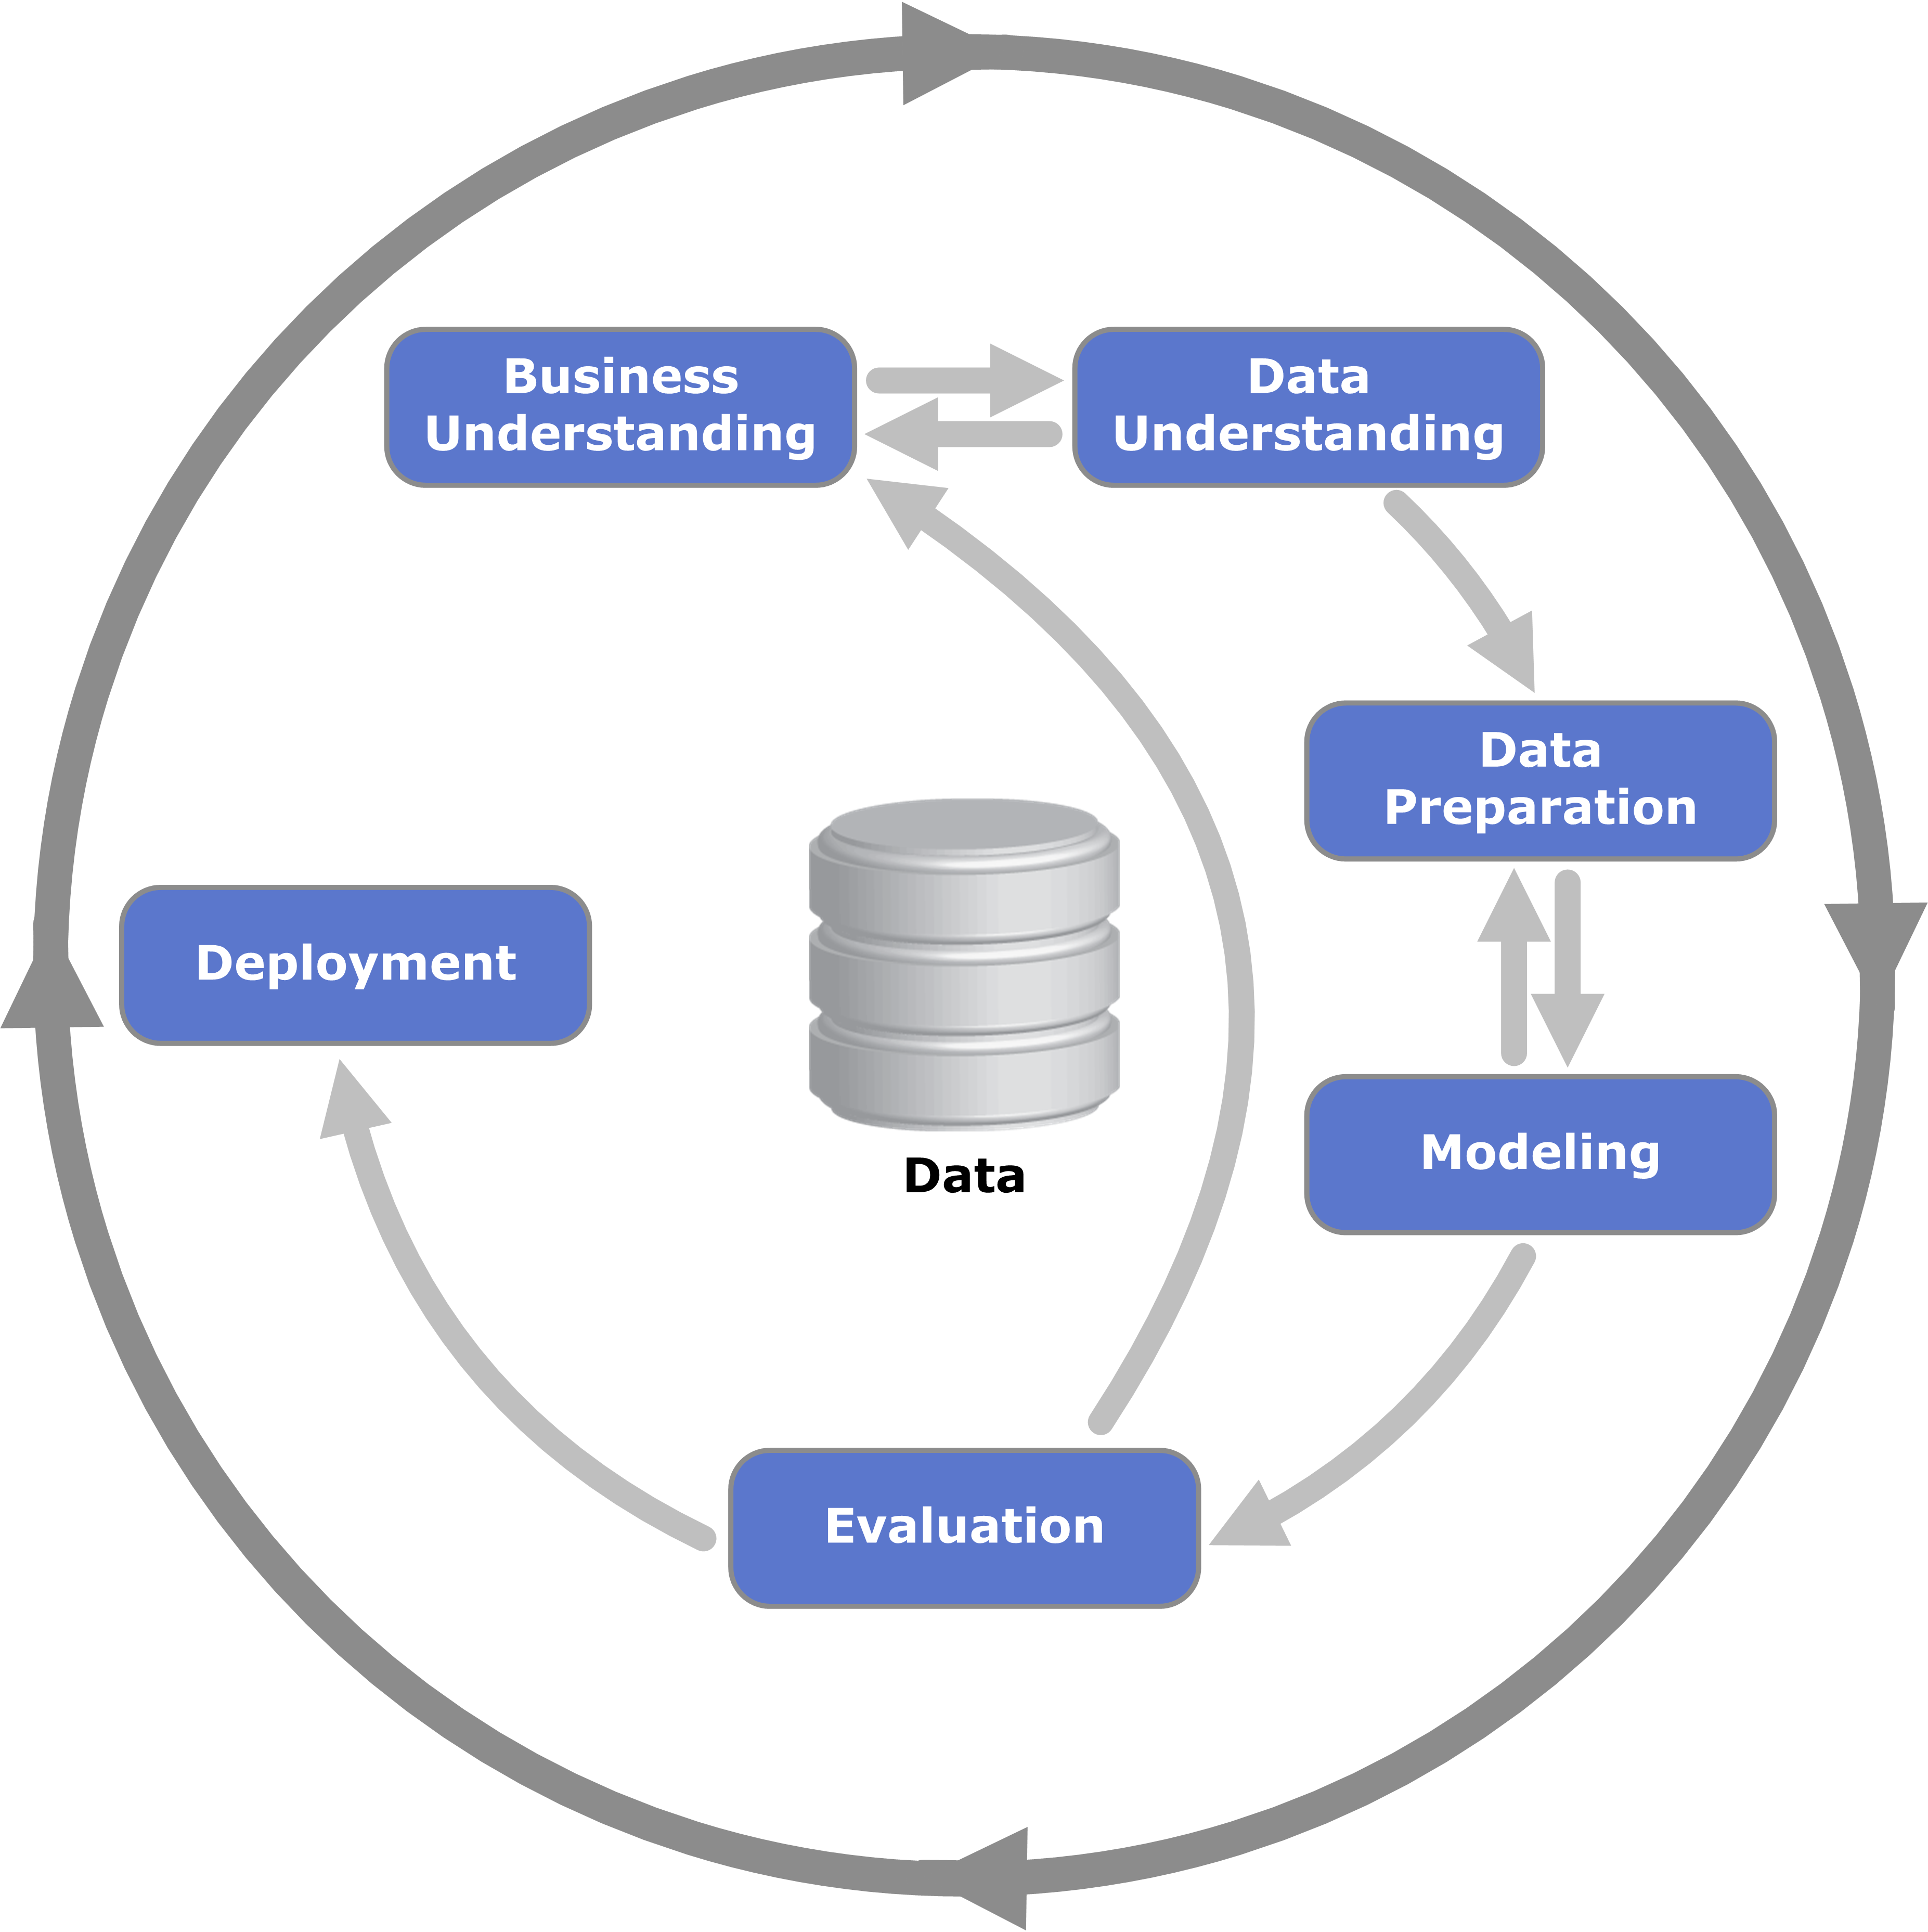
\includegraphics[width=0.5\linewidth]{./images/CRISP-DM.png}
	\caption{CRISP-DM}
	\label{fig:crispdm}
\end{figure}

\subsubsection{Business Understanding}
Utilizing obstacle detection with computer vision can play a crucial role in helping various enterprises address concerns with regards to safety. Companies that focus in industries such as autonomous vehicles, railroads, and robotics can use this idea to detect any obstacles in real time. This helps prevent severe accidents from occurring. It also allows drivers to focus on the road without having to also detect whether anything comes in the way. Having this extra safety mechanism can help to increase a human's trust and reliability on the product if using something like autonomous vehicles since it ensures the customer that extra safety precautions are being taken. If accidents occur, time and money must be spent for repairs, while at the same time inconveniencing unrelated parties. Having a quick and accurate obstacle detection mechanism in place can identify potential obstacles and help prevent accidents from occurring.


\subsubsection{Data Understanding}
For the data collection phase, the primary datasets will be sourced from public repositories such as the COCO dataset, RoboFlow, and other APIs that are focused on obstacle detection across various domains (Mainly on Autonomous Vehicle). The custom datasets will also be created and used by capturing images and videos in various environments.

For the data exploration phase, we are going to conduct an initial EDA process to assess the distribution of the class, such as car, pedestrian, and more. Another important aspect of our data that we need to understand is its format. For example, YOLOv8 and GroundingDINO can use JPEG and PNG images with JSON annotations, while Detectron2 supports JPEG, PNG, and TIFF image formats, also using JSON annotations. It is essential that the data format is known, because the data will be combined into one master dataset. One issue that arises when doing so is differing formats among the data. As stated before, certain architectures are able to handle certain image types, label formats, etc. Additionally, data often come in different formats, such as image size, colorspace, image type, and annotation format. Due to this, we must understand the data formats first to ensure consistency when we combine our data together.


\subsubsection{Data Preparation}
The dataset can consist of a set of images or videos. Since our datasets will be combined into one master dataset, the data must be consistent across all datasets. For any videos in the dataset, we can convert them into images by splitting it into frames. Then, we will resize the images to be the same size, as differing sizes will cause issues with modeling. Next, we will ensure each image is in the same colorspace by changing the color representation so that each pixel is either in a black and white format or in an RGB (Red, Green, Blue) scale representation. Additionally, we will convert all of the images to the majority image type.

Once this is done, the data can be preprocessed to increase robustness, as well as to increase the model's performance.
Images within the dataset can be cropped to eliminate parts that are irrelevant to the detection process. Rotation and flipping will be applied to obtain additional training data in different orientations. We will try normalizing certain pixel values which can help keep the components of the image on one scale and help the model reach the optimal solution faster. In case any unnecessary components are discovered, we can apply masking so the model only focuses on the relevant parts. In a similar project using YOLOv8 to detect moving objects conducted by \textcite{safaldin_improved_2024}, preprocesses a video, by decoding it which required them to ``isolate each frame from the video'', making adjustments to the size of each frame since ``YOLO architectures require certain input sizes'', and adjusting the color by transforming ``pixel values to a range between to [0, 1] or [-1, 1]'' depending on the model used.

% *** https://docs.opencv.org/4.x/d2/d96/tutorial_py_table_of_contents_imgproc.html *** this just has some stuff that opencv can do in terms of image preprocessing

\subsubsection{Modeling}

In the model selection phase, the project is primarily implemented by three different well-known object detection model architectures, which are YOLOv8, Detectron2, and GroundingDINO. The YOLO architecture is a popular real-time object detection model with high speed and accuracy, which makes it suitable for a real-time detection application. Detectron2 is developed by Facebook AI Research, and the main advantage is the flexibility of selecting various backbone networks and the robustness of the model performance. Finally, GroundingDINO is a transformer-based architecture that shows strong performance in visual grounding tasks.

During the model training phase, these selected architectures will be trained and optimized for the obstacle detection tasks outlined in the project. Initially, transfer learning will be utilized by leveraging weights from a pre-trained model that have been trained on larger datasets such as COCO. This will allow models to preserve some important features while reducing the time and data required for training. Additionally, fine tuning these models may be required depending on the performance.



\subsubsection{Evaluation}
To evaluate the performance of each model, there are different techniques available to use. To compare the effectiveness of each YOLO model, \textcite{quach_evaluating_2023} utilize measurement scales such as Average Precision (AP) to help identify how well the model detects various objects. They also other standard evaluation metrics such as precision, recall, and F1-score to determine the model's performance in order to identify with how much certainty it can classify a certain image. Their evaluations are based on an ``Intersection of Union threshhold (IoU) or ground truth ratio to confirm whether the recognized object is true or false'' \parencite{quach_evaluating_2023}. We will obtain the precision, recall, and f1-scores to evaluate the model performance. Using the precision values, we will also calculate the mean average precision. This metric is considered as the ``consolidated metric for assessing model accuracy across varying categories and confidence levels'' \parencite{safaldin_improved_2024}. Alongside that, we will determine the Intersection of Union to determine how much similarity there is between the actual label and the predicted label.

\subsubsection{Deployment}
The product deployment will consist of the model that detects obstacles and objects the most accurately. The model will be trained on a dataset containing autonomous vehicles which would accurately detect if there are any obstacles or objects present if the car is in motion.


\subsection{Data Pipeline Architecture}
% data sources, data warehouse, ETL, ELT, data transfers with pipeline, and deliverables

% data source aside, do we even have a start for the other steps
For this project, the image data and labels will be sourced from previously established datasets with research, such as the COCO dataset, as well as more targeted data from online aggregates like Roboflow. This data will then be stored in an AWS S3 bucket. For ETL and pipelining, we will focus on extracting the data from the bucket, transforming them to a single format (image type, image size, colorspace, etc.), then loading it into the data warehouse.

\subsection{Project Organization Plan}
To organize the project, a work breakdown structure was creating by decomposing the project hierarchically and incrementally into phases, deliverables, and work packages. The phases, deliverables, and work packages are as follows:

\begin{enumerate}
	\item Business Understanding: This phase is split into four main work packages: Defining the problem, performing literature and technology surveys on the topic, determining the data source, and creating the project plan framework.

	\item Data Understanding: This phase it split into two packages: Understanding the image data and initial exploratory data analysis. Understanding the image data is a hierarchical system, where the sub packages involves understanding the format of the data, as well as understanding the images themselves in terms of factors such as image size, colorspace, and image type.

	\item Data Preparation: This phase involves two packages: Preparing the data and Splitting the data. Preparing the data is split up into various, incremental tasks: Collecting the data, reformatting the data to be consistent with each other, cleaning the data, transforming and augmenting the data, and labeling the data if needed. Once this is done, we can split the data into train, validation, and testing sets.

	\item Modeling: The modeling phase has 3 main packages: Model Research, Modeling and Validation, and Evaluation. Model Research is split into 3 sub tasks: researching YOLOv8, Detectron2, and GroundingDINO. Once this is completed we can move on to the modeling and validation step, where these architectures will go through transfer learning and fine tuning. Finally, we can evaluate the models by comparing their performances, and select the best performing one.

	\item Deployment: The deployment phase has two deliverables: Deploying the project and data onto AWS as a backend prototype, and the final report submission.
\end{enumerate}

The work breakdown structure can be seen in Figure \ref{fig:wbs}.
\begin{figure}[!htb]
	\centering
	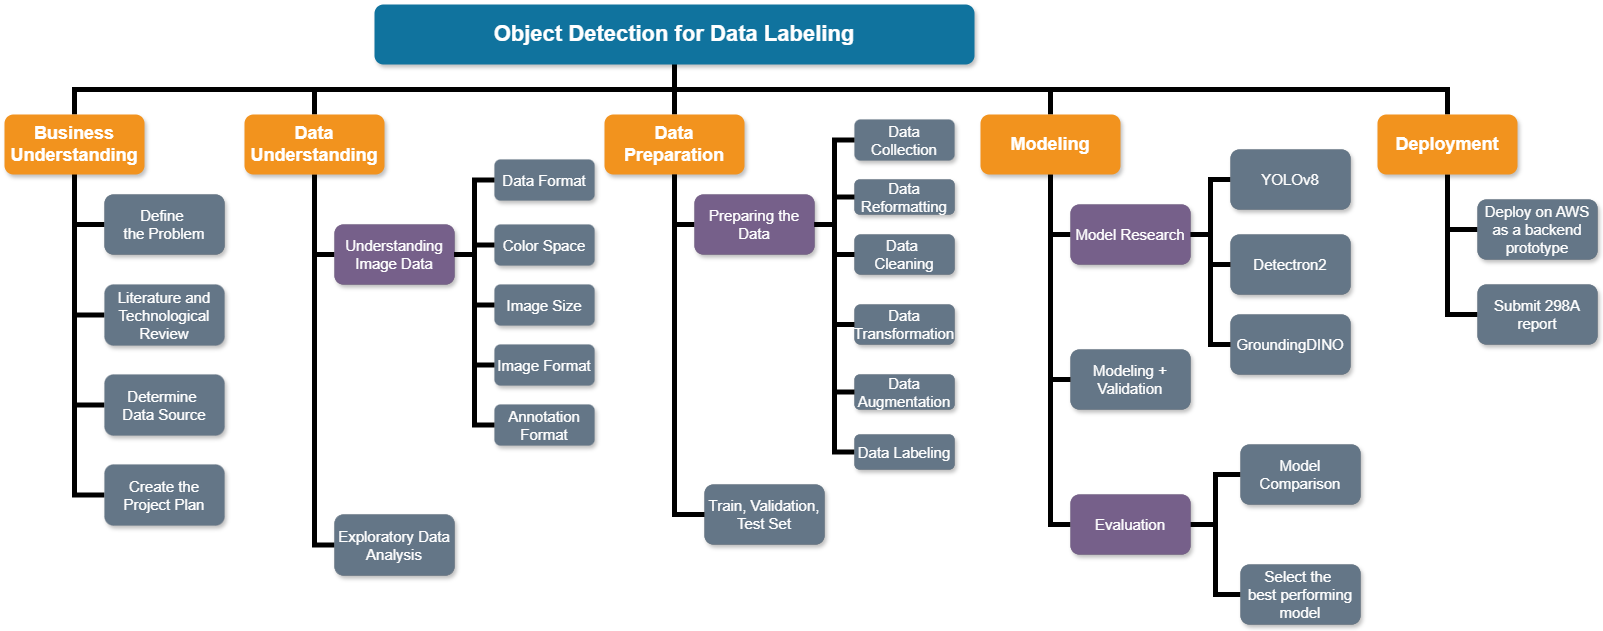
\includegraphics[width=1\linewidth]{./images/WBS_updated.png}
	\caption{Work Breakdown Structure}
	\label{fig:wbs}
\end{figure}


\subsection{Project Resource Requirements and Plan}
\subsubsection{Hardware}
Deep learning is generally computationally intensive, especially when performing it on images. As a result, we require more powerful hardware. The main pieces of hardware we plan to utilize are our own local machines and Google Colab. A summary of our hardware requirements can be seen in Table \ref{tab:hardware}.

We plan on utilizing Google Colab for initial testing. Google Colab is a free-to-use, cloud-based Jupyter Notebook with access to GPU and TPU resources. The free-to-use version has limited resources, so depending on the process, a paid plan may be required. Additionally, Google Colab is integrated with Google Drive, allowing data storage and collaboration through the use of shared drives.

\begin{table}[!htb]
	\centering
	\caption{Hardware Requirements}
	\begin{tabular}{cccc}
		\hline
		Service        & Configuration     & Purpose          & Cost         \\
		\hline
		Local Machines & various           & Coding platform  & Owned (free) \\
		Google Colab   & T4 GPU (16GB RAM) & Compute platform & Free         \\
		\hline
	\end{tabular}
	% \tablenote{*Paid version available, A100 GPU utilizes approximately 11 compute units/hour}
	\label{tab:hardware}
\end{table}

\subsubsection{Software}
To preprocess the data and create the models, various software tools must be utilized. The primary coding language will be Python. In addition to Python, various libraries and modules related to modeling and data preprocessing will be used. We also use GitHub and Google Colab for collaborative coding, and Google Docs and Overleaf for report writing A comprehensive list of the software used can be seen in Table \ref{tab:software}.

There are no specific licenses require for the aforementioned tools and platforms. The majority of these tools are open-source, or have free versions for both personal and academic use. Businesses and organizations may have different requirements such as having to purchase licenses, but this does not apply for our use case.

\begin{table}[!htb]
	\centering
	\caption{Software Requirements}
	\begin{tabular}{cccc}
		\hline
		Service          & Configuration  & Purpose                      & Cost      \\
		\hline
		Python           & Version 3.11   & Coding platform              & Free      \\
		Pandas           & Version 2.1.1  & Working with datasets        & Free      \\
		NumPy            & Version 1.26.1 & Advanced mathematics         & Free      \\
		PyTorch          & Version 2.4    & Modeling, Data Preprocessing & Free      \\
		OpenCV           & Version 4.10   & Image Processing             & Free      \\
		Ultralytics      & Version 8.3.2  & Modeling (with YOLOv8)       & Free      \\
		Detectron2       & Version 0.6    & Modeling (with Detectron2)   & Free      \\
		Jupyter Notebook & Version 6.5.4  & Code REPL platform           & Free      \\
		Google Colab     & N/A            & Code REPL platform           & Free      \\
		Kaggle Notebook  & N/A            & Code REPL platform           & Free      \\
		GitHub           & N/A            & Code collaboration           & Free      \\
		Overleaf         & N/A            & Report writing collaboration & \$9/month \\
		TeamGantt        & N/A            & Gantt charts                 & Free      \\
		\hline
	\end{tabular}
	% \tablenote{*Paid version available}
	\label{tab:software}
\end{table}

\subsection{Project Schedule}

Project management is required to make sure projects are completed on time. To do so we use the waterfall technique to task management and to keep up with it we are following a schedule. This schedule can be visualized as a Gantt chart or PERT chart. A Gantt chart (see figure \ref{fig:gantt} and \ref{fig:gantt2}) shows the tasks on a timeline with dependencies, resources, and durations clearly visible. It allows for quick references to make sure we are on track. A PERT chart (see figure \ref{fig:pert}) allows us to find the critical path in a projects completion. If there is a delay in any of the tasks in the critical path, that means there will be a delay on the entire project.

\printbibliography

\appendix

\section{Project Management Charts}
\begin{figure}
	\centering
	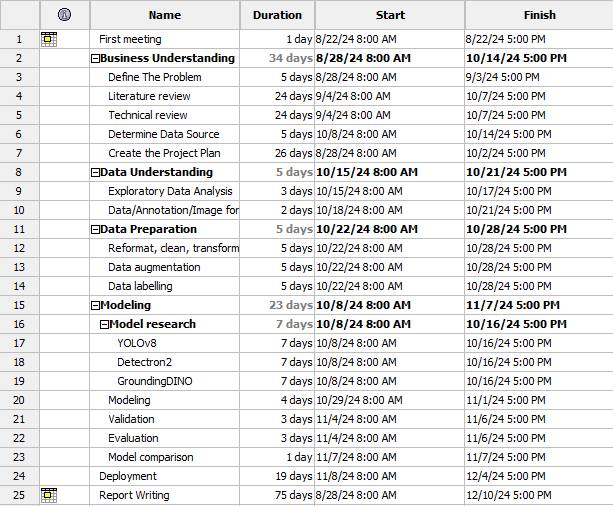
\includegraphics[width=\linewidth]{images/gantt/gantt1.png}
	\caption{Gantt Chart details}
	\label{fig:gantt}
\end{figure}
\begin{figure}
	\centering
	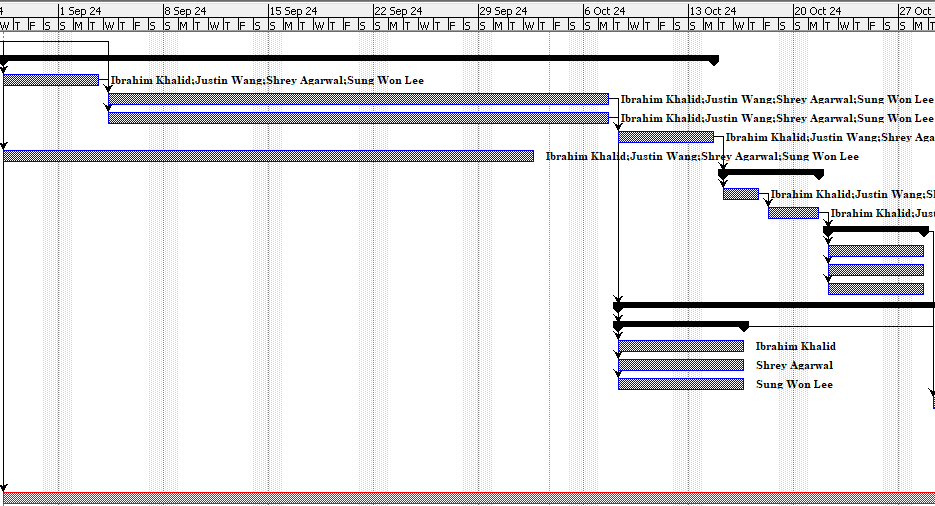
\includegraphics[width=\linewidth]{images/gantt/gantt2.png}
	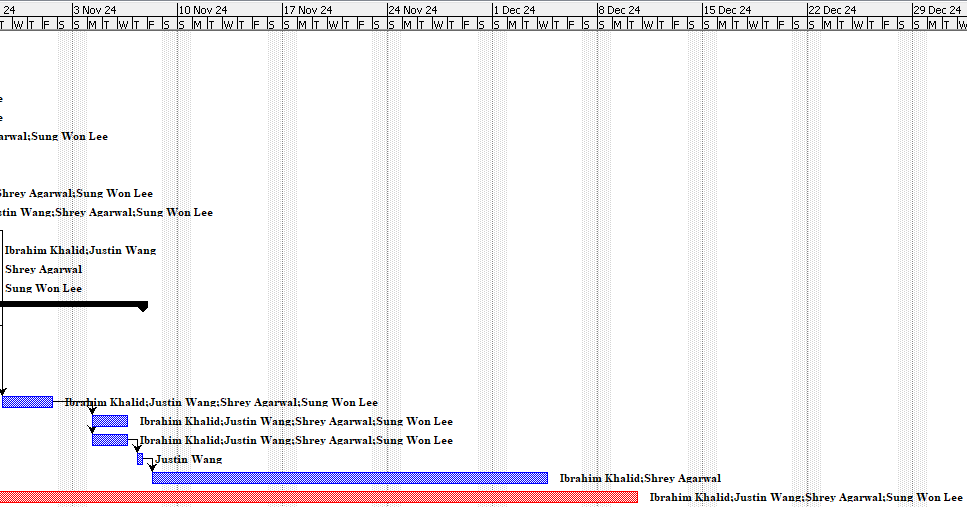
\includegraphics[width=\linewidth]{images/gantt/gantt3.png}
	\caption{Gantt Chart Calendar view}
	\label{fig:gantt2}
\end{figure}

\begin{figure}
	\centering
	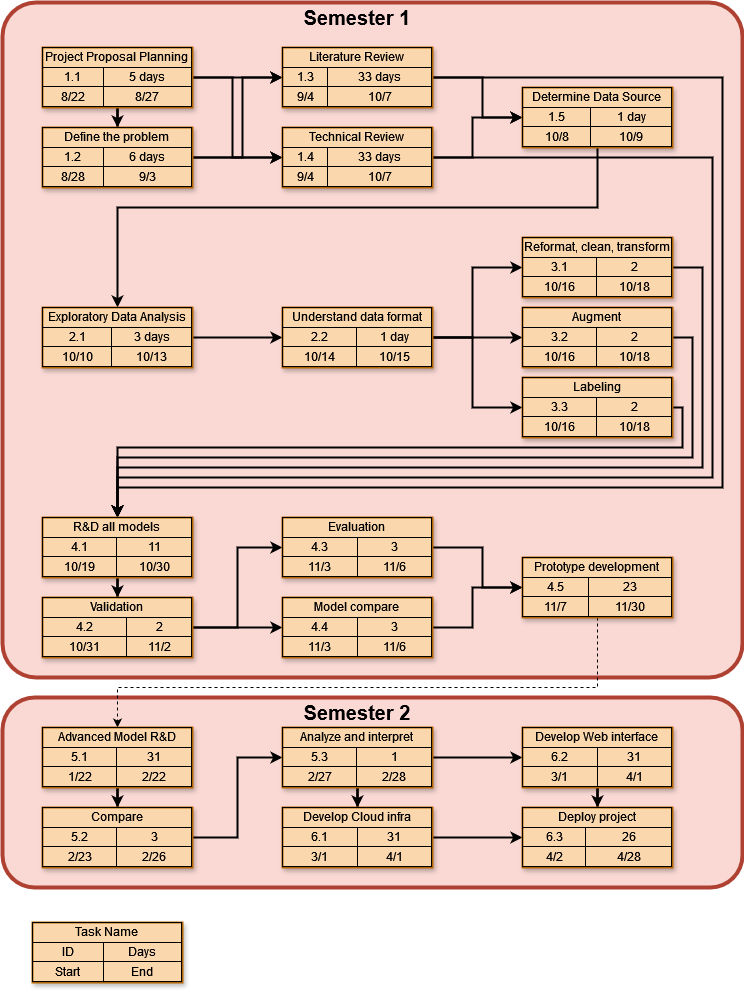
\includegraphics[width=\linewidth]{images/pert.png}
	\caption{PERT chart}
	\label{fig:pert}
\end{figure}

\end{document}